\chapter{Números (1º Bimestre)}

\section{Conjuntos numéricos e Números irracionais}

\subsection*{Resumo}

Os números reais (designoados por $\mathbb R$) podem ser representados como
pontos em uma reta.

\begin{center}
\begin{tikzpicture}
  \draw (-3,0) --(3,0);
  \path (-4,0) node (minf) {$\ldots$};
  \path (4,0) node (inf) {$\ldots$};
  \draw (-1,-.1) --(-1,.1);
  \draw (-2,-.1) --(-2,.1);
  \draw (0,-.1) --(0,.1);
  \draw (1,-.1) --(1,.1);
  \draw (2,-.1) --(2,.1);
  \path (0,.5) node (n0) {$0$};
  \path (1,.5) node (n1) {$1$};
  \path (2,.5) node (n2) {$2$};
  \path (-1,.5) node (nm1) {$-1$};
  \path (-2,.5) node (nm2) {$-2$};
\end{tikzpicture}
\end{center}

Os números naturais (designados por $\mathbb N$) são $0, 1, 2, 3, \ldots$. Se
também incluirmos os números negativos, obteremos os números inteiros
(designados por $\mathbb Z$: $\ldots, -3, -2, -1, 0, 1, 2, 3, \ldots$).
Os números da forma $\frac{p}{q}$ onde $p \in \mathbb Z$ e $q \in \mathbb N
\setminus \{0\}$ são chamados de racionais (designados por $\mathbb Q$). Em
particular, se considerarmos os números decimais onde $q = 10^n$ para algum $n
\in \mathbb N$, obteremos os números decimais como $-494,1627$.
Os reais que não são racionais são chamados de irracionais.

\begin{center}
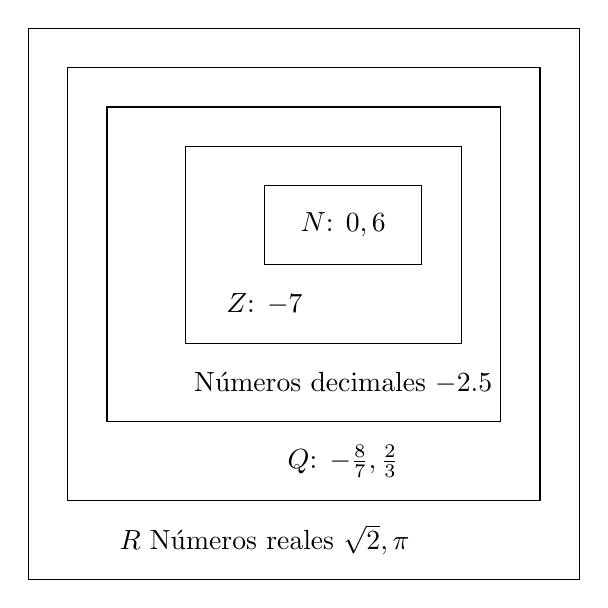
\begin{tikzpicture}
  \draw (0,0) rectangle(7,7);
  \path (3,0.5) node (R) {$\mathbb R$ Números reales $\sqrt{2}, \pi$};
  \draw (.5,1) rectangle(6.5,6.5);
  \path (4,1.5) node (Q) {$\mathbb Q$: $-\frac{8}{7}, \frac{2}{3}$};
  \draw (1,2) rectangle(6,6);
  \path (4,2.5) node (D) {Números decimales $-2.5$};
  \draw (2,3) rectangle(5.5,5.5);
  \path (3,3.5) node (Z) {$\mathbb Z$: $-7$};
  \draw (3,4) rectangle(5,5);
  \path (4,4.5) node (N) {$\mathbb N$: $0, 6$};
\end{tikzpicture}
\end{center}

\subsection*{Exemplos}

\begin{enumerate}
  \item $364$ é um número natural.
  \item $-36$ é um número inteiro (negativo) mas não é um número natural.
  \item $0.8$ é um número decimal mas não é inteiro.
  \item $\frac{1}{3}$ é um número racional mas não é um número decimal.
  \item $\sqrt{2}$ é um número real mas não é um número racional
  (see BraFunMat7, bimestre 1, exercise 8).
\end{enumerate}

\subsection*{Exercício 1}

Calcule $3n$ e $3{(n+1)}$ para $n = 3, 33, 333, 3333\ldots$ e $10^m$ para
$m = 0, 1, 2, 3, \ldots$.

Suponhamos que $\frac{1}{3}$ pode ser escrito como um decimal
$\frac{n}{10^m}$ onde $n \in \mathbb N$ e $m \in \mathbb N$. Isso é possível?

\subsection*{Exercício 2}

Classifique os números a seguir.

\begin{enumerate}
\item $6$
\item $-2$
\item $2.5$
\item $-7.0$
\item $\frac{3}{2}$
\item $-\frac{1}{3}$
\item $\frac{16}{8}$
\item $\sqrt{2}$
\item $\sqrt{49}$
\item $\sqrt{\frac{16}{25}}$
\item $\sqrt[3]{0.125}$
\end{enumerate}

\subsection*{Exercício 3}

Marque na reta numérica os números: $0, 1, 8,
0.25, -4, \frac{9}{4}, \frac{10}{3}, -\sqrt{2}$.

\subsection*{Exercício 4 (Número de Euler)}

Para todo $n \geq 1$, temos
$$e_n = \sum_{k=0}^{n} \frac{1}{k!}$$
onde $k! = 1 \times 2 \times 3 \times \ldots \times k$ e
$$f_n = 2 + \sum_{k=2}^{n} \frac{1}{2^{k-1}}$$

\begin{enumerate}
\item Calcule $f_n - 2$ para $n = 1, 2, 3, 4$.
  O que você pode afirmar sobre os números $f_n$?
\item Compute $e_n$ para $n = 1, 2, 3, 4$. O que você pode afirmar sobre esses
  números?
\item Compare $k!$ e $2^{k-1}$ para $k \geq 3$ e deduza uma comparação para
  $e_n$ e $f_n$ para $n \geq 3$.
\item Iremos ver em uma seção futura que $e_n$ aproxima-se de um número real
  denotado por $e$ a medida que $n$ cresce. $e$ pode ser um número inteiro?
\item Suponha que podemos encontrar inteiros $a,b$ tais que
  $b > 1$ e $e = \frac{a}{b}$ seja um racional. Definimos
  $x = b!\left(e - e_b\right)$. Mostre que $x > 0$ e que ele é um inteiro.
\item Para todo $n \geq b$ temos
  $x_n = b!\left(e_n - e_b\right)$ que aproxima-se de $x$ ao aumentarmos o valor
  de $n$. Então
  $$x_n = \sum_{k=b+1}^{n} \frac{1}{{(b+1)} \times {(b+2)} \times {(b+3)}
    \times \ldots \times k}$$
\item Definimos para todo $n \geq b$
  $$y_n = \sum_{k=1}^n \frac{1}{\left(b+1\right)^k}$$
  Determine $\left(1 - \frac{1}{b+1} \right) y_n$ e deduza que
  $y_n < \frac{1}{b}$.
\item Compare $x_n$ e $y_n$ e deduza que $x<1$. Depois disso escreva suas
  conclusões.
\end{enumerate}

\section{Potenciação e radiciação}

Se $r$ é um número real e $n$ é um inteiro, então já definimos na 7ª série $r^n$
para o caso em que $r \neq 0$ ou $n \neq 0$.

Se $r \geq 0$ e $n > 0$ é um inteiro, então existe um único real $s \geq 0$ tal
que $s^n = r$. Chamamos $s$ da $n$-ésima raiz de $r$ e denotamos por
$s = \sqrt[n]{r}$.
Note que $\left(-s\right)^n = \left(-1\right)^n s^n = \left(-1\right)^n r$.
Podemos definir raízes de números negativos pela fórmula
$\sqrt[n]{-r} = -s = -\sqrt[n]{r}$
quando $n$ é ímpar mas não temos uma fórmula para quando $n$ é par
pois nesse último caso qualquer potência de $n$ é não negativa.

Considere $r > 0$.
Se $n > 0$,
definimos
$r^{\frac{1}{n}} = \sqrt[n]{r}$
tal que
$\left(r^{\frac{1}{n}}\right)^n = 1$.
De forma similar, se $m$ é outro inteiro não zero,
definimos 
$r^{\frac{m}{n}} = \left(\sqrt[n]{r}\right)^m = \left(r^{\frac{1}{n}}\right)^m$
para ser consistente com a lei das potências usuais.
Isso define potências racionais para qualquer número real positivo.
No futuro iremos generalizar isso para números irracionais.

\subsection*{Exercício 5}

Calcule as seguintes potências e raízes:

\begin{enumerate}
\item $\left(-3\right)^5$
\item $\sqrt[3]{27}$
\item $12^3$
\item $\sqrt[3]{1.728}$
\item $\left(-0.00243\right)^{\frac{1}{5}}$
\item $\sqrt[4]{160000}$
\item $20^3$
\item $160000^{0.75}$
\item $243^{0.8}$
\item $125^{\frac{2}{3}}$
\end{enumerate}

\section{Notação científica}

Qualquer número real $r$ pode ser escrito na forma
$$r = a \times 10^b$$
para um número real $1 \leq \left|a\right| < 10$ e $b$ inteiro.
Por exemplo, $1,23 \times 10^{-3}$ ou $-3,981 \times 10^{7}$.
Esse notação permite representar de forma concisa qualquer número muito grande,
por exempo $23049497292000000000 = 2.3049497292 \times 10^{19}$,
ou números muito pequenos,
por exemplo $0.0000000000000382 = 3.82 \times 10^{-15}$,
e compará-los facilmente.

\subsection*{Exercício 6}

Coloque os números abaixo em notação científica e depois ordene-os.

\begin{enumerate}
\item $a=123$
\item $b=230000000000$
\item $c=0.000000002$
\item $d=11 \times 10^-7$
\item $e=\frac{1}{4}$
\item $f=-2\times 10^5$
\end{enumerate}

\section{Solução dos exercícios}

\subsection*{Exercício 1}

Obtemos $9, 99, 9999, 99999$, $12, 102, 1002, 10002$ e
$1, 10, 100, 1000, 10000, \ldots$.
Notamos que $10^m$ nunca é divisível por $3$.
Então $\frac{1}{3} = \frac{n}{10^m}$ não é possível pois caso contrário teríamos
$10^m = 3n$.

\subsection*{Exercício 2}

\begin{enumerate}
\item $6$ é um número natural.
\item $-2$ é um número inteiro mas não é natural.
\item $2.5 = \frac{25}{10^1}$ é um número decimal mas não é inteiro.
\item $-7.0 = -7$ é um número inteiro mas não é natural.
\item $\frac{3}{2} = 1.5$ é um número decimal mas não é inteiro.
\item $-\frac{1}{3}$ é um numero racional mas não é decimal (ver exercício 1).
\item $\frac{16}{8} = 2$ é um número natural.
\item $\sqrt{2}$ é um numero real mas não é racional (ver exercício 3).
\item $\sqrt{49} = 7$ é um número natural.
\item $\sqrt{\frac{16}{25}} = \frac{4}{5} = \frac{8}{10^1} = 0.8$ é um número
decimal mas não é inteiro.
\item $\sqrt[3]{0.125} = 0.5$ é um número decimal mas não é inteiro.
\end{enumerate}

\subsection*{Exercício 3}

$0.25 = \frac{1}{4}$, $\frac{9}{4} = 2 + \frac{1}{4}$,
$\frac{10}{3} = 3 + \frac{1}{3}$, $-\sqrt{2} \approx -1.414213562373095$

\begin{center}
\begin{tikzpicture}
  \draw (-9,0) --(9,0);
  \draw (1,-.2) --(1,.2);
  \draw (2,-.1) --(2,.1);
  \draw (3,-.1) --(3,.1);
  \draw (4,-.1) --(4,.1);
  \draw (5,-.1) --(5,.1);
  \draw (6,-.1) --(6,.1);
  \draw (7,-.1) --(7,.1);
  \draw (8,-.1) --(8,.1);
  \draw (0,-.2) --(0,.2);
  \draw (-1,-.1) --(-1,.1);
  \draw (-2,-.1) --(-2,.1);
  \draw (-3,-.1) --(-3,.1);
  \draw (-4,-.1) --(-4,.1);
  \draw (-5,-.1) --(-5,.1);
  \draw (-6,-.1) --(-6,.1);
  \draw (-7,-.1) --(-7,.1);
  \draw (-8,-.1) --(-8,.1);
  \path (0,.5) node (n0) {$0$};
  \path (1,.5) node (n1) {$1$};
  \path (2,.5) node (n2) {$2$};
  \path (3,.5) node (n3) {$3$};
  \path (4,.5) node (n4) {$4$};
  \path (-4,.5) node (nm4) {$-4$};

  \draw (0.25,-.1) --(0.25,2);
  \draw (0.5,-.1) --(0.5,.1);
  \draw (0.75,-.1) --(0.75,.1);
  \path (0.25,2.2) node (n025) {$0.25$};

  \draw (2.25,-.1) --(2.25,2);
  \path (2.25,2.2) node (n94) {$\frac{9}{4}$};

  \draw (3.333333333333,-.1) --(3.333333333333,2);
  \draw (3.666666666666,-.1) --(3.666666666666,.1);
  \path (3.333333333333,2.2) node (n103) {$\frac{10}{3}$};

  \draw (-1.414213562373095,-.1) --(-1.414213562373095,2);
  \path (-1.414213562373095,2.2) node (nmsqrt2) {$-\sqrt{2}$};


\end{tikzpicture}
\end{center}

\subsection*{Exercício 4 (Número de Euler)}

\begin{enumerate}
\item $f_1 - 2 = 0$, $f_2 - 2 = \frac{1}{2}$,
  $f_3 - 2 = \frac{3}{4}$, $f_4 - 2 = \frac{7}{8}$
  e em geral vemos que
  $f_n$ é um sequência crescente de números menores que $3$
  que aproxima-se cada vez mais de $3$.

\item $e_1 = \frac{1}{1} + \frac{1}{1} = 2$, $e_2 = e_1 + \frac{1}{2!} = 2.5$
  $e_3 = e_1 + \frac{1}{3!} = \frac{8}{3} = 2.66666666666\ldots$ e
  $e_4 = e_3 + \frac{1}{4!} = \frac{65}{24} \approx
  2.708333333333333$.
  Eles formam uma sequência crescente de números maiores ou igual a 2 sendo que
  o crescimento é cada vez menor (pois em cada passo é adicionado o valor
  $\frac{1}{n!}$ que decresce quando $n$ aumenta).
\item Para $k > 3$,
  $k! = 1 \times 2 \times 3 \times 4 \times \ldots \times k >
  1 \times
  \underset{k-1\,\text{vezes}}{\underbrace{2 \times 2 \times \ldots \times 2}} =
  2^{k-1}$.
  Como uma consequencia $\frac{1}{k!} < \frac{1}{2^{k-1}}$
  e para $n \geq 3$ temos
  $$
  2 <
  e_n = 2 + \sum_{k=2}^{n} \frac{1}{k!}
  <
  f_n = 2 + \sum_{k=2}^{n} \frac{1}{2^{k-1}} < 3
  $$

\item Pelo exercício anterior,
  temos que $2 < e < 3$ e portanto ele não pode ser inteiro.

\item Encontramos que
  $x = b!\left(\frac{a}{b} - \sum_{k=0}^{b}\frac{1}{k!} \right)
  = a \left(b-1\right)! - \sum_{k=0}^{b} {{(k+1)} \times {(k+2)} \times
    {(k+3)} \times \ldots \times b} \in \mathbb Z$
  Além disso, temos $e_0 < e_1 < e_2 < \ldots < e_b < e_{b+1} < \ldots < e$
  de modo que $x = b!\left(e - e_b\right) > 0$.

\item Temos que
$$x_n = b!\left(e_n - e_b\right)
 = \sum_{k=0}^n \frac{b!}{k!} - \sum_{k=0}^{b} \frac{b!}{k!}
 = \sum_{k=b+1}^n \frac{b!}{k!}
 = \sum_{k=b+1}^{n} \frac{1}{{(b+1)} \times {(b+2)} \times {(b+3)}
    \times \ldots \times k}
$$

\item Encontramos que
$\left(1 - \frac{1}{b+1}\right) y_n =
{\sum_{k=1}^n \frac{1}{\left(b+1\right)^k}}
- {\sum_{k=1}^n \frac{1}{\left(b+1\right)^{k+1}}} =
\frac{1}{b+1} - \frac{1}{\left(b+1\right)^{n+1}} < \frac{1}{b+1}$.
Como consequência, $y_n < \frac{\frac{1}{b+1}}{1 - \frac{1}{b+1}}
= \frac{1}{b+1-1} = \frac{1}{b}$.

\item Temos que $x_n \leq y_n < \frac{1}{b}$ para todo $n \geq b$ e logo
  $x \leq \frac{1}{b} < 1$.
  Mas então $x$ seria um inteiro tal que $0 < x < 1$!
  Por essa contradição, deduzimos que $e$ não é um racional.

\end{enumerate}

\subsection*{Exercício 5}

\begin{enumerate}
\item $\left(-3\right)^5 = -3^5 = -9 \times 9 \times 3 = -81 \times 3 = -243$
\item $\sqrt[3]{27} = \sqrt[3]{3 \times 9} = \sqrt[3]{3 \times 3 \times 3} = 3$
\item $12^3 = 144 \times 12 = 1728$
\item $\sqrt[3]{1.728} =
  \left(\frac{1728}{1000}\right)^{\frac{1}{3}} =
  \frac{1728^{\frac{1}{3}}}{1000^{\frac{1}{3}}} =
  \frac{12}{10} = 1.2$
\item $\left(-0.00243\right)^{\frac{1}{5}} =
  -\left(\frac{243}{100000}\right)^{\frac{1}{5}} =
  -\left(\frac{3^5}{10^5}\right)^{\frac{1}{5}} =
  -\frac{3}{10} = -0.3$
\item $\sqrt[4]{160000} = \left(2^4 \times 10^4\right)^{\frac{1}{4}} = 20$
\item $20^3 = 2^3 \times 10^3 = 8000$
\item $160000^{0.75} = 160000^{\frac{3}{4}} = \sqrt[4]{160000}^3 = 20^3 = 8000$
\item $243^{0.8} = 243^{\frac{4}{5}} = \sqrt[5]{243}^4 = 3^4 = 9^2 = 81$
\item $125^{\frac{2}{3}} = \sqrt[3]{5^3}^2 = 5^2 = 25$
\end{enumerate}

\subsection*{Exercício 6}

\begin{enumerate}
\item $a = 1.23 \times 10^2$
\item $b = 230000000000 = 2.3 \times 10^{11}$
\item $c = 2 \times 10^{-9}$
\item $d = 1.1 \times 10^{-6}$
\item $e = 0.25 = 2.5 \times 10^{-1}$
\item $f = -2\times 10^5$ (já em notação científica)
\end{enumerate}

Temos então que $f < c < d < e < a < b$.
